\begin{figure}[!h]
\centering
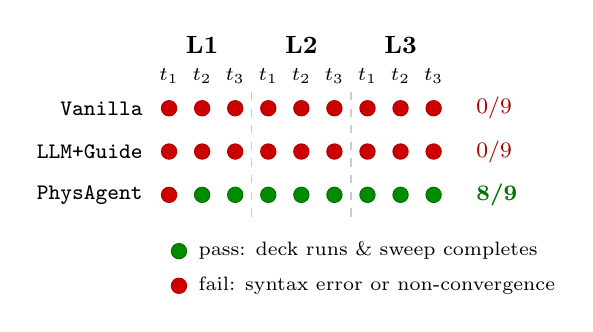
\begin{tikzpicture}[
    x=0.42cm, y=0.55cm,
    font=\footnotesize,
    passdot/.style={circle, draw=green!45!black, fill=green!55!black, inner sep=0pt, minimum size=5.5pt},
    faildot/.style={circle, draw=red!70!black,   fill=red!80!black,   inner sep=0pt, minimum size=5.5pt},
    opendot/.style={circle, draw=red!70!black,   fill=white, thick,   inner sep=0pt, minimum size=5.5pt},
]
    % Level group labels
    \node[font=\small\bfseries] at (1,3.45) {L1};
    \node[font=\small\bfseries] at (4,3.45) {L2};
    \node[font=\small\bfseries] at (7,3.45) {L3};

    % Trial tick labels (t1 t2 t3 repeated)
    \foreach \gx in {0,3,6}{
      \foreach \t/\dx in {$t_1$/0, $t_2$/1, $t_3$/2}
        \node[font=\scriptsize] at (\gx+\dx, 2.75) {\t};
    }

    % Row labels (left)
    \node[anchor=east, font=\footnotesize\ttfamily] at (-0.5, 2) {Vanilla};
    \node[anchor=east, font=\footnotesize\ttfamily] at (-0.5, 1) {LLM+Guide};
    \node[anchor=east, font=\footnotesize\ttfamily] at (-0.5, 0) {PhysAgent};

    % Row: Vanilla (no_source)  -- all fail
    \foreach \x in {0,1,2,3,4,5,6,7,8}
      \node[faildot] at (\x, 2) {};

    % Row: LLM+Guide (manual_mmd_subset) -- all fail
    \foreach \x in {0,1,2,3,4,5,6,7,8}
      \node[faildot] at (\x, 1) {};

    % Row: PhysAgent (ontology_mcp) -- L1_t1 fail, rest pass
    \node[faildot] at (0, 0) {};
    \foreach \x in {1,2,3,4,5,6,7,8}
      \node[passdot] at (\x, 0) {};

    % Right-side summary
    \node[anchor=west, red!65!black,  font=\footnotesize] at (9.0, 2) {0/9};
    \node[anchor=west, red!65!black,  font=\footnotesize] at (9.0, 1) {0/9};
    \node[anchor=west, green!45!black,font=\footnotesize\bfseries] at (9.0, 0) {8/9};

    % Separators between L1/L2/L3 groups (dashed)
    \draw[gray!40, dashed] (2.5,-0.5) -- (2.5,2.5);
    \draw[gray!40, dashed] (5.5,-0.5) -- (5.5,2.5);

    % Legend (below, stacked)
    \node[passdot] at (0.3,-1.3) {};
    \node[anchor=west, font=\scriptsize] at (0.6,-1.3) {pass: deck runs \& sweep completes};
    \node[faildot] at (0.3,-2.1) {};
    \node[anchor=west, font=\scriptsize] at (0.6,-2.1) {fail: syntax error or non-convergence};
\end{tikzpicture}
\caption{Per-trial TCAD execution on Si nMOSFET across prompt-detail levels L1/L2/L3 and trials $t_1$--$t_3$. A trial passes only if Sentaurus parses the generated deck without syntax errors and the Id--Vg sweep completes. Vanilla and LLM+Guide fail on every trial---predominantly at parse time---while PhysAgent passes 8/9.}
\label{fig:exp1}
\end{figure}
